% ------------------------------------------------------------------------------
% TYPO3 Version 10.1 - What's New (Serbian Version)
%
% @license	Creative Commons BY-NC-SA 3.0
% @link		https://typo3.org/help/documentation/whats-new/
% @language	Serbian
% ------------------------------------------------------------------------------

\section{Uvod}
\begin{frame}[fragile]
	\frametitle{Uvod}

	\begin{center}\huge{Uvod}\end{center}
	\begin{center}\huge{\color{typo3darkgrey}\textbf{Činjenice}}\end{center}

\end{frame}

% ------------------------------------------------------------------------------
% TYPO3 Version 10.1 - The Facts

\begin{frame}[fragile]
	\frametitle{Uvod}
	\framesubtitle{TYPO3 Verzija 10.1 - Činjenice}

	\begin{itemize}
		\item Datum objavljivanja: 01. oktobar 2019
		\item Tip objavljivanja: Brza objava (Sprint Release)
	\end{itemize}

	\begin{figure}
		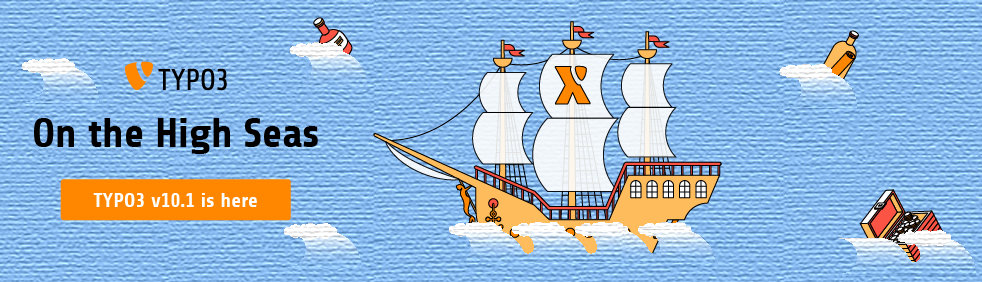
\includegraphics[width=0.95\linewidth]{Introduction/typo3-v10-1-banner.png}
	\end{figure}

\end{frame}

% ------------------------------------------------------------------------------
% TYPO3 Version 10.1 - Executive Summary

\begin{frame}[fragile]
	\frametitle{Uvod}
	\framesubtitle{Rezime}

	\small
		TYPO3 verzija 10.1 je druga brza objava na putu ka LTS-verziji
		(verzija sa dugoročnom podrškom) u 2020.

		\vspace{0.2cm}

		Nova objava sadrži više od 240 git komita (pregledane, testirane i
		odobrene izmene na kodu) od kada je prethodna verija 10.0 objavljena pre
		deset nedelja.

		\vspace{0.2cm}

		Iako korisnici administratorskog interfejsa neće videti previše izmena ili
		novih funkcionalnosti, TYPO3 10.1 donosi mnoga poboljšanja "ispod haube".

	\normalsize

\end{frame}

% ------------------------------------------------------------------------------
% System Requirements

\begin{frame}[fragile]
	\frametitle{Uvod}
	\framesubtitle{Sistemski zahtevi}

	\begin{itemize}
		\item PHP verzija 7.2 ili 7.3
		\item PHP podešavanja:

			\begin{itemize}
				\item \texttt{memory\_limit} >= 256M
				\item \texttt{max\_execution\_time} >= 240s
				\item \texttt{max\_input\_vars} >= 1500
				\item opcija \texttt{-}\texttt{-disable-ipv6} \underline{ne sme} se koristit
			\end{itemize}

		\item Većina DB servera koji rade sa \textbf{Doctrine DBAL} rade takodje i sa TYPO3.
			Testirani DB serveri su:
	\end{itemize}

	\begin{figure}
		
\includegraphics[width=0.80\linewidth]{Introduction/logo-databases.png}
	\end{figure}

\end{frame}

% ------------------------------------------------------------------------------
% Development, Release and Maintenance Timeline

\begin{frame}[fragile]
	\frametitle{Uvod}
	\framesubtitle{Razvoj, objavljivanje i vreme održavanja}

	\textbf{TYPO3 v10}

	\begin{figure}
		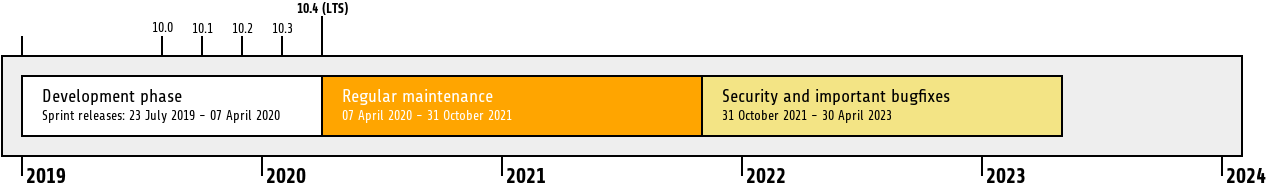
\includegraphics[width=1\linewidth]{Introduction/typo3-v10-lifecycle.png}
	\end{figure}

	\textbf{Produženo vreme podrške}\newline
	\smaller
		\href{https://typo3.com}{TYPO3 GmbH} nudi dodatne opcije za podršku za
		TYPO3 v10 LTS čak i posle 30. Aprila 2023. za dodatne dve godine.
	\normalsize

\end{frame}

% ------------------------------------------------------------------------------
% TYPO3 v10 Roadmap

\begin{frame}[fragile]
	\frametitle{Uvod}
	\framesubtitle{TYPO3 v10 plan}

	Predvidjeni datumi objavljivanja i njihov osnovni fokus:

	\begin{itemize}

		\item v10.0 \tabto{1.1cm}23/July/2019\tabto{3.4cm}Otvaranje puta za uzbudljive nove koncepte i API-je
		\item
			\begingroup
				\color{typo3orange}
				v10.1 \tabto{1.1cm}01/Oct/2019\tabto{3.4cm}Unapredjenje routing-a i upravljanje sajtom v2
			\endgroup
		\item v10.2 \tabto{1.1cm}03/Dec/2019\tabto{3.4cm}Fluid/Rendering Engine unapredjenja
		\item v10.3 \tabto{1.1cm}04/Feb/2020\tabto{3.4cm}Zamrzavanje funkcionalnosti
		\item v10.4 \tabto{1.1cm}07/Apr/2020\tabto{3.4cm}LTS objava (objava sa dugoročnom podrškom)

	\end{itemize}

	\smaller
		\url{https://typo3.org/article/typo3-v10-roadmap/}\newline
		\url{https://typo3.org/article/typo3-v10-safe-and-sound/}
	\normalsize

\end{frame}

% ------------------------------------------------------------------------------
% Installation

\begin{frame}[fragile]
	\frametitle{Uvod}
	\framesubtitle{Instalacija}

	\begin{itemize}
		\item Zvanična \textit{klasična} procedura za instalaciju na Linux/Mac OS X\newline
			(DocumentRoot na primer \texttt{/var/www/site/htdocs}):
		\begin{lstlisting}
$ cd /var/www/site
$ wget --content-disposition get.typo3.org/10.1
$ tar xzf typo3_src-10.1.0.tar.gz
$ cd htdocs
$ ln -s ../typo3_src-10.1.0 typo3_src
$ ln -s typo3_src/index.php
$ ln -s typo3_src/typo3
$ touch FIRST_INSTALL
		\end{lstlisting}

		\item Simbolički linkovi (Symbolic links) na Microsoft Windows:

			\begin{itemize}
				\item Koristiti \texttt{junction} za Windows XP/2000
				\item Koristiti \texttt{mklink} za Windows Vista, Windows 7 i novije
			\end{itemize}

	\end{itemize}
\end{frame}

% ------------------------------------------------------------------------------
% Installation using composer

\begin{frame}[fragile]
	\frametitle{Instalacija i ažuriranje}
	\framesubtitle{Instalacija korišćenjem \texttt{composer-a}}

	\begin{itemize}
		\item Instalacija korišćenjem \textit{composer-a} na Linux/Mac OS X i Windows 10:

			\begin{lstlisting}
$ cd /var/www/site/
$ composer create-project typo3/cms-base-distribution typo3v10 ^10.1
			\end{lstlisting}

		\item Alternativno, napravite Vaš \texttt{composer.json} fajl i pokrenite:

			\begin{lstlisting}
$ composer install
			\end{lstlisting}

			Više detalja i primer \texttt{composer.json} fajla možete skinuti sa:\newline
			\smaller
				\href{https://composer.typo3.org}{https://composer.typo3.org}
			\normalsize

	\end{itemize}
\end{frame}

% ------------------------------------------------------------------------------
